\documentclass{article}

\usepackage{url}
\usepackage{microtype}
\usepackage{parskip}
\usepackage[super]{natbib}
\usepackage[a4paper, left=2.5cm, right=2.5cm, top=2.5cm, bottom=2.5cm]{geometry}
\usepackage{longtable,booktabs}
\usepackage{caption}
\usepackage{blindtext}
\usepackage{graphicx}
\usepackage{authblk}
\usepackage{amsmath}
\usepackage{lineno}
\usepackage[toc,page]{appendix}
\usepackage[utf8]{inputenc}
\usepackage{array} %for the tables in appendix
\usepackage{tabularx} %for the tables in appendix

\usepackage{multicol}
\setlength{\columnsep}{5mm} %column separation

%working title...
\title{Automated visual representation of service use for clients diagnosed with a personality disorder, using timelines and Python.\\
\vspace{0.5cm}
%\large{A practical framework to visualise service use as timelines using Python.}}
}
\author[1]{*Kerry Pearn}
\author[1]{Sean Manzi}
\author[2]{Lindsay Winterton}

\affil[1,*]{\footnotesize University of Exeter Medical School \& NIHR South West Peninsula Applied Research Collaboration (ARC).}
\affil[2]{\footnotesize Devon Partnership Trust, National Health Service, UK}
\affil[*]{\footnotesize Corresponding author: k.pearn@exeter.ac.uk}

\begin{document}

\maketitle

\section*{Abstract} 

\emph{Background and motivation}: Clients with a personality disorder diagnosis accessing mental health services do not follow a predefined linear care pathway. As a result, clients are allocated one or more of a large number of services available to them at any one time. It becomes increasingly important for clinicians to understand clients past treatment to inform future decisions so as to provide a care pathway that is suitable for them. Clinicians in Devon (South West England) currently access information of a client’s service use history in the form of a traditional static tabular presentation. This paper presents an alternative visualisation of the client’s service use data (Service Use Timelines) that will reduce the clinicians time and effort to extract the meaningful and relevant information.

\emph{Method}: Create Python code for automated parsing of client records to create a visual representation of a single clients service use history in the form of a timeline.

\emph{Results}: We demonstrate how the program may be used to create a visual representation of the clients service use history in the form of a timeline, from routinely collected service use data.

\emph{Conclusion}: Python code has been developed and shared to enable a visual representation of the clients service use history. Here we share a description of the development process and links to full Python code.

\emph{GitHub repository of code and dataset}: \url{https://github.com/kerrypearn/service_use_timelines}

\section*{Keywords}
Mental health services; visualisation; service improvement; personality disorder
%\begin{multicols}{2}

\section{Introduction}

A personality disorder (PD) is a mental health diagnosis for a collection of conditions where an individual behaves, thinks, feels or relates to others very differently from the average person \cite{NHS}. These traits often make it difficult for the individual to live with themselves and/or other people, in addition, these individuals are not able to change their problematic traits \cite{RoyalCollegeofPsychiatrists2015}. In 2006, a UK study suggested that about 1 in 22 people will have a PD at a given time \cite{Coid2006}, which equates to 3.0 million people in the UK \cite{OfficeforNationalStatistics2017}. Clients with a PD diagnosis have historically been deemed as “untreatable”, with targetted psychological treatment only becoming available since 1990 when clinical trials showed that some of these psychological treatments had some effect \cite{Pollack1990, LinehanMMArmstrongHESuarezAAllmonD1991}. Treatment currently available in England for clients with a PD diagnosis include psychological or medicinal treatment, as well as offering the necessary support, acknowledging that treatment needs to be tailored to the client as no single approach suits everyone \cite{NHS}. Since publication of NMIHE 2003 guidelines \cite{NationalInstitueforMentalHealthinEngland2003} a specialist PD service has been made available in most, but not all, UK trusts. In 2015, 84\% of English mental health trusts had a dedicated PD service \cite{Dale2017}. Despite this, issues remain for the care pathway of clients with PD diagnosis as the care pathway is unclear for both clinicians and service users  \cite{FlynnSRaphaelJGraneyJNyathiTWilliamsAKapurNApplebyLShaw2019}. In addition, clients with a PD diagnosis (Borderline) identified that there is a lack of knowledge and understanding around the diagnosis, which coupled with the lack of resources available, they felt that staff relied on pharmacological intervention \cite{Rogers2011}, when this should only be administered in times of crisis. Improvements to the care pathway for clients diagnosed with a PD are still required, and this is reflected in the Royal College of Psychiatrists Position Statement “Services for people diagnosable with personality disorder” \cite{RoyalCollegeofPsychiatrists2020} which, in January 2020, outlined the need to implement a whole pathway approach where clients flow through linked up services. This is yet to be implemented, but is an encouraging future vision and aim for the care pathway.

Individual care pathways over the course of a client's treatment can vary greatly in complexity between clients. This becomes apparent from the onset as their first contact can originate from a large number of services. Aside from mental health services, these can also include: general practitioners, drug and alcohol services, criminal justice system, secondary care emergency services, social services, being homeless and sleeping rough \cite{Bolton2014}. Once in the system clients can be referred to a variety of services at any given time, but without a particular order. This can result in cyclical pathways. These are instances when clients move back and forth between services without a specific direction or long-term treatment goal. Improving understanding of a client’s service use history and treatment trajectory could help clinicians define long-term treatment goals and avoid cyclical pathways.

In Devon (county in South West England), the specialist PD service is delivered by Devon Partnership Trust (DPT). DPT use Carenotes database to collate service use history \cite{Advanced}. Clinicians can access this information in a traditional tabular format, figure \ref{fig:carenotes}. This format makes it hard to extract the overall history of the clients services use and define an overview of their treatment pathway.

This is not a problem specific to the treatment of PD, other services have found similar issues. A visualisation technique – timelines \cite{Cousins1991} – has been used to display client service use history. Timelines use a continuous horizontal line to depict a duration of service use, with the x axis displaying the date and y axis displaying the service used, This technique has already been applied to numerous electronic health datasets in the NHS, such as dementia \cite{Carey2016},  primary health care services received by care home residents \cite{Goodman2013} and Hospital Episode Statistics \cite{England2013}.

Clinicians agree that timelines provide a succinct and streamlined view of client service use history, which could provide them with benefits, particularly in client safety, quality of care and better support their cognitive processes (compared to their current clinical computer systems) \cite{Gill2010}. It has been demonstrated that displaying client service use history as timelines (rather than a tabular record) led to faster response times (for date/interval comparisons and making intercategorical connections), reduce some “first impressions” biases and had a higher recall in a memory test \cite{Alonso1998}, whilst also improving the understanding of the clinical data and helping complex patterns to be recognised in the data \cite{Ledesma2019}.

In this paper we present 1) a PD service use dataset, 2) the visual representation of the dataset in the form of individual client Service Use Timelines (SUT), and 3) provide a link to Python code for automated parsing of client records to create a SUT for each client in the anonymised Carenotes dataset. The code extends that provided by \url{https://sukhbinder.wordpress.com/2016/05/10/quick-gantt-chart-with-matplotlib/}, and the timeline visualisation is based on that published by Cousins S, Kahn M (1991)\cite{Cousins1991}. 

\begin{figure}[!h]
	\centering
	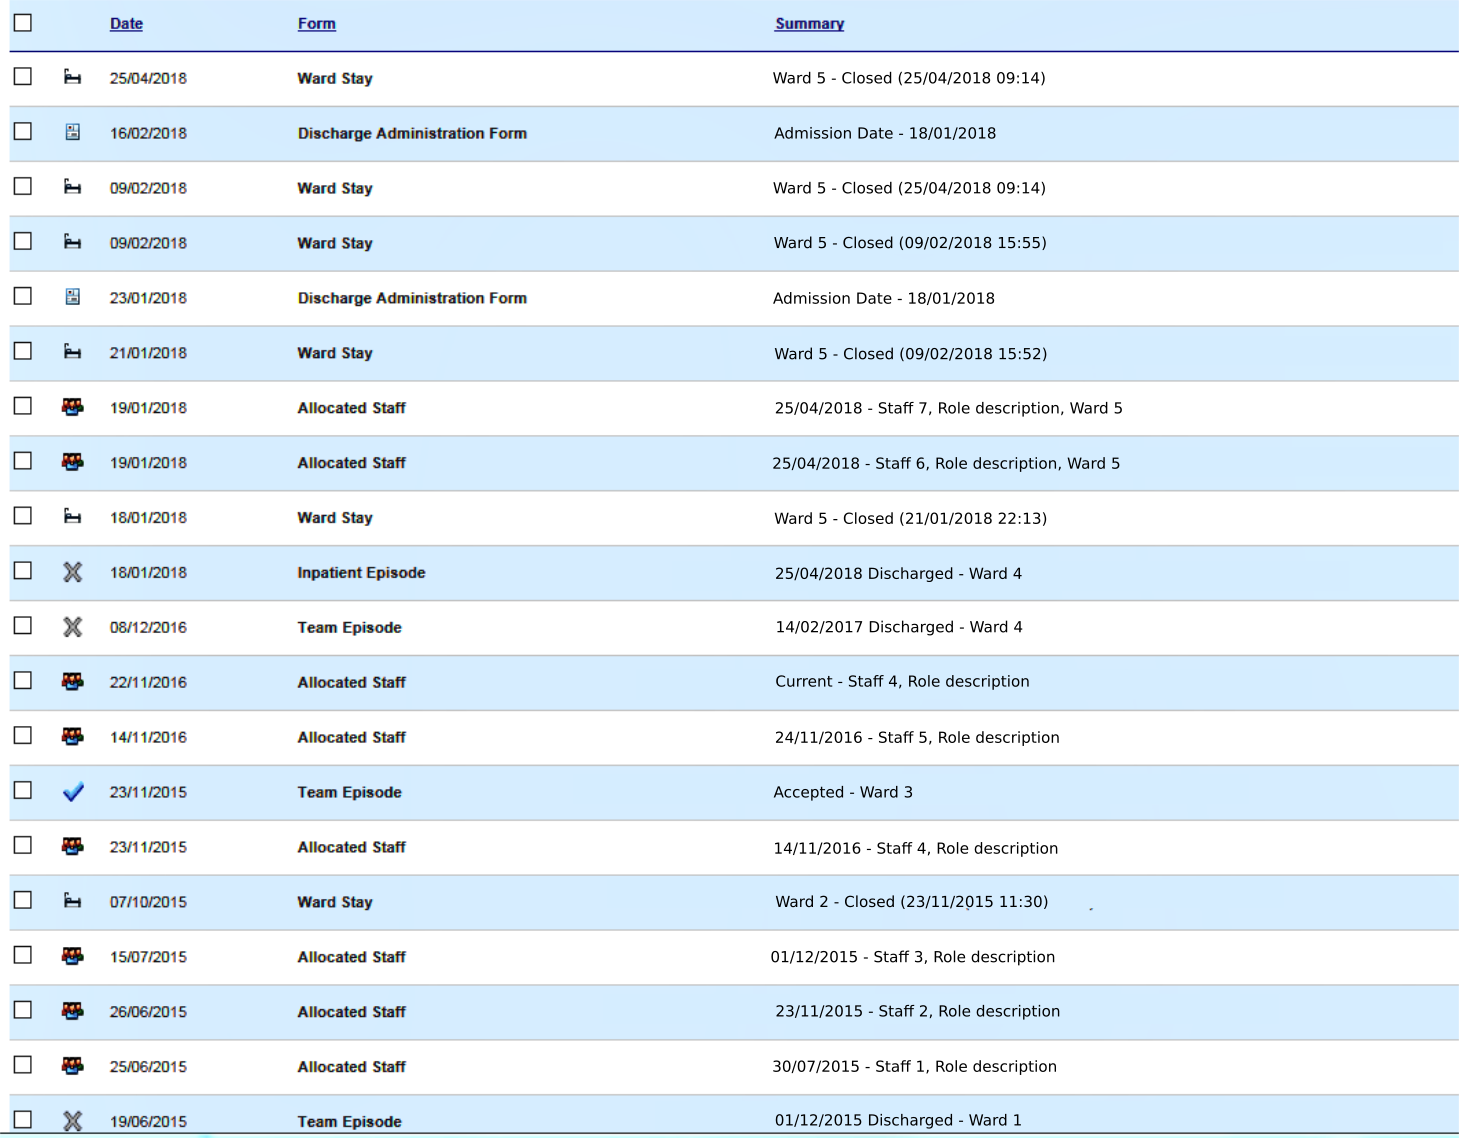
\includegraphics[width=0.9\textwidth]{images/Carenotes_screenshot_anonymous.png}
\caption{Screen shot of the Carenotes display showing an individual client’s service use in a traditional tabular format (data has been anonymised). This is the current way clinicians view client service use data.}
	\label{fig:carenotes}
\end{figure}

\section{GitHub repository}

The GitHub repository containing this code and an anonymised PD service use dataset is:

\url{https://github.com/kerrypearn/service_use_timelines}

\section{Method}

\subsection{The dataset}

Carenotes is an electronic client record system that is widely used by NHS Trusts to record client’s community, mental health and child health service use \cite{Advanced,BlueFrontier}. It is designed to support clinicians to plan, manage, record and analyse their client care. Records include diagnoses, services accessed, client characteristics and referral source.

\subsection{Population identification}
The sample dataset used for the development of the SUT included all service use episodes from 01/01/2015 until 18/02/2018 for any client diagnosed with a PD (defined as a client with any one of the following twelve ICD-10 diagnostic codes: F60, F600, F601, F602, F603, F604, F605, F606, F607, F608, F609, F61 or being in mental health care cluster 7 or 8. See Appendix for code descriptions). The sample dataset contained 13 variables to describe the client and their service use (see Appendix for full list and description). 

\subsection{Data cleaning assumptions}
For the purposes of this model development exercise, episodes with a missing value for referral date were removed from the dataset. Episodes with a missing discharge date were interpreted as ongoing service, and therefore imputed with the extraction date (18 Feb 2018). Errors in data entry where the discharge occurred before the referral were also removed.

\subsection{Consultations with clinical staff}
Development of the SUT included an interactive process with care providers to ensure that the tool was fit for purpose. We convened a group of DPT staff, including clinicians, nurses, managers, informatics analysts and administration. The feedback process included four separate feedback consultations which helped to identify which variables to include in the SUT, and how best to display them.

\subsection{The code}
Coded in Python, extending the example code provided by \url{https://sukhbinder.wordpress.com/2016/05/10/quick-gantt-chart-with-matplotlib/}.
The SUT’s are created using the matplotlib library. We also use the following libraries: numpy, pandas and datetime. For each unique client in the sample dataset, a matplotlib graphic of the SUT is created and saved in a svg format. Figure \ref{fig:process_diagram} shows the process diagram of the main steps in the code.

\begin{figure}[!h]
	\centering
	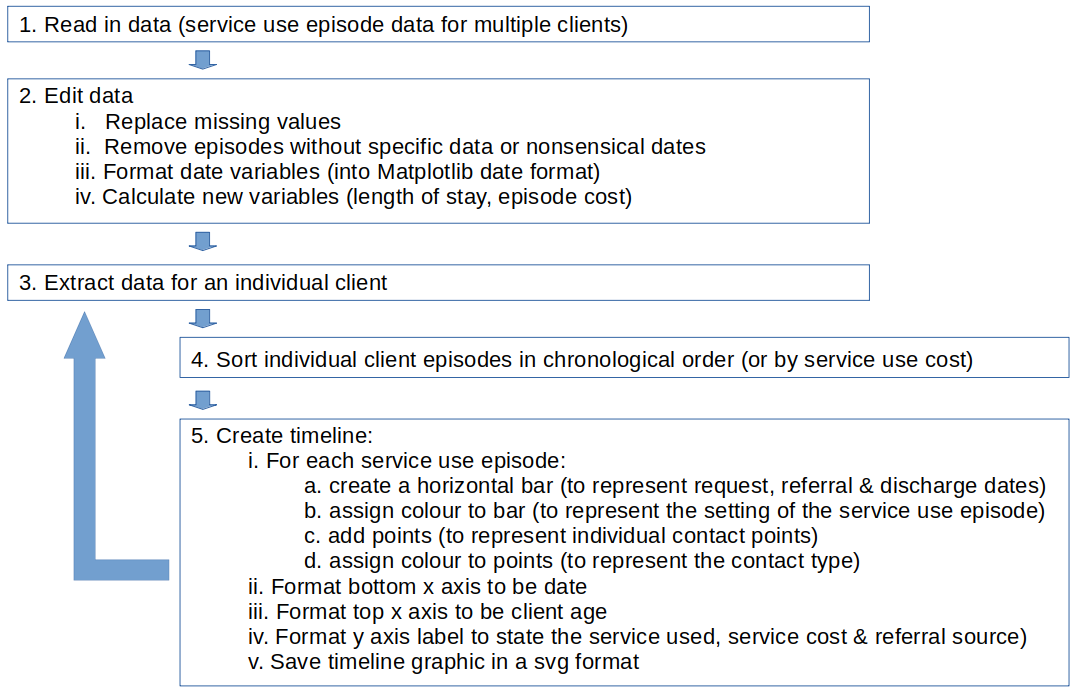
\includegraphics[width=0.9\textwidth]{images/process_diagram.png}
	\caption{Steps taken in the Python code to create a timeline visualisation from Carenotes dataset.}
	\label{fig:process_diagram}
\end{figure}

\section{Results}

\subsection{Population description}
We identified 6631 unique clients with a diagnosis of PD using services between 01/01/2015 and 18/02/2018. These clients accessed a total of 229 unique care services. In this 3 year period, each client accessed on average 5.6 services (standard deviation 6.0, median 4, range 1 to 95). In total, the sample dataset contains 37,281 service use episodes. A care service is used on average 161.4 times (standard deviation 374.4, median 21, range 1 to 3080). The clients’ age at referral is on average 38.8 yrs old (standard deviation 15.6, median 36, range 14.6 to 99.8). The average duration of service use is 153.1 days (standard deviation 298.5 days, median 21 days, range 0 to 1,854 days).

\subsection{Consultation process}
During the feedback consultations, DPT staff helped to inform the visual representation of the SUT. The feedback could be grouped into three main points:
\begin{itemize}
	\item \emph{Skewed representation of service use intensity}: The long length of stays for some community services highlighted the need to use another variable to give a better context of the amount of resource used. This is due to some clients being allocated to a particular service for years with very few contacts, compared to an intensive month program where contacts would be weekly. The SUT would also display individual contacts to give the service use episode a better context of resource use.
	\item \emph{Request for additional variables}: Four additional variables (to those included in the sample Carenotes dataset) were requested to be displayed on the SUT.  The information analysts at DPT identified that three of the variables are currently recorded in the full Carenotes dataset (and so could easily be included in a future data extraction), these were: date of individual contacts, contact type, and date of decision to refer client to a service. One variable is not yet recorded in Carenotes and so would require additional data collection: service cost. For the purpose of this model development exercise, we included mock values for the additional four variables requested so that they could be included in the visualisation development. 
	\item \emph{Tailoring categories}: DPT staff requested that some of the levels used for the categorical variables be tailored to suit their purposes. For example, for service setting and service locality to each have a separate category to represent whether a service is a Psychiatric Intensive Care Unit (PICU), regardless of whether this was an out of area resource.
\end{itemize}

\subsection{The code}
Coded in Python, and is available at \url{https://github.com/kerrypearn/service_use_timelines}

\subsection{Service use timeline graphic}
SUT’s are a visual support tool to aid clinician makes decisions on the treatment of PD. The display aims to provide a concise description of the complete service use history based on data collected in Carenotes, where use of each particular service is represented by a horizontal bar, as shown in figure \ref{fig:sut}. 
\begin{itemize}
	\item \emph{x-axis}: represents time. Time is characterised as both the date (the bottom axis) and by the client’s age, (the top axis). 
	\item \emph{y-axis}: displays the service the client was referred to. The default view displays used services on the y-axis by chronological order based on the referral date (with the earliest at the top). However, this can be tailored to suit several purposes (for example, services can be ordered by cost, length of stay, decision to admit date, or grouped by setting). Each service use instance on the y-axis is identified by a text field, which can be comprised of multiple text strings so as to tailor the description given for each episode. We currently include the name of the team providing the service, the source of the referral and the cost of the service use episode. The geographic locality of the service is displayed using colour coding of the text on the y-axis text label, as seen in the bottom left of figure \ref{fig:sut}.
	\item \emph{horizontal bars}: represent the duration for which a client was waiting for and admitted to a service based on their   care records. The grey section of the bar represents waiting time for the service (this is the time from the decision to admit the client - when a clinician has registered the referral, until the referral date - the start of a service use). The coloured portion of the bar represents length of stay for that service (this is the time from the date of referral until discharge). The colour of the bar represents the setting (community, inpatient, out of area, PICU). 
	\item \emph{points}: located within each horizontal bar and represent individual contacts with the service. Their symbology discriminates between type of contact (e.g. face-to-face or by other means).
	\item \emph{title and footnote}: additional information about the client is given in the title (such as unique ID, ICD-10 code and mental health cluster code). The footnote is used to expand on any of this information (such as the description of the ICD-10 code) and list any assumptions used.
\end{itemize}

\begin{figure}[!h]
	\centering
	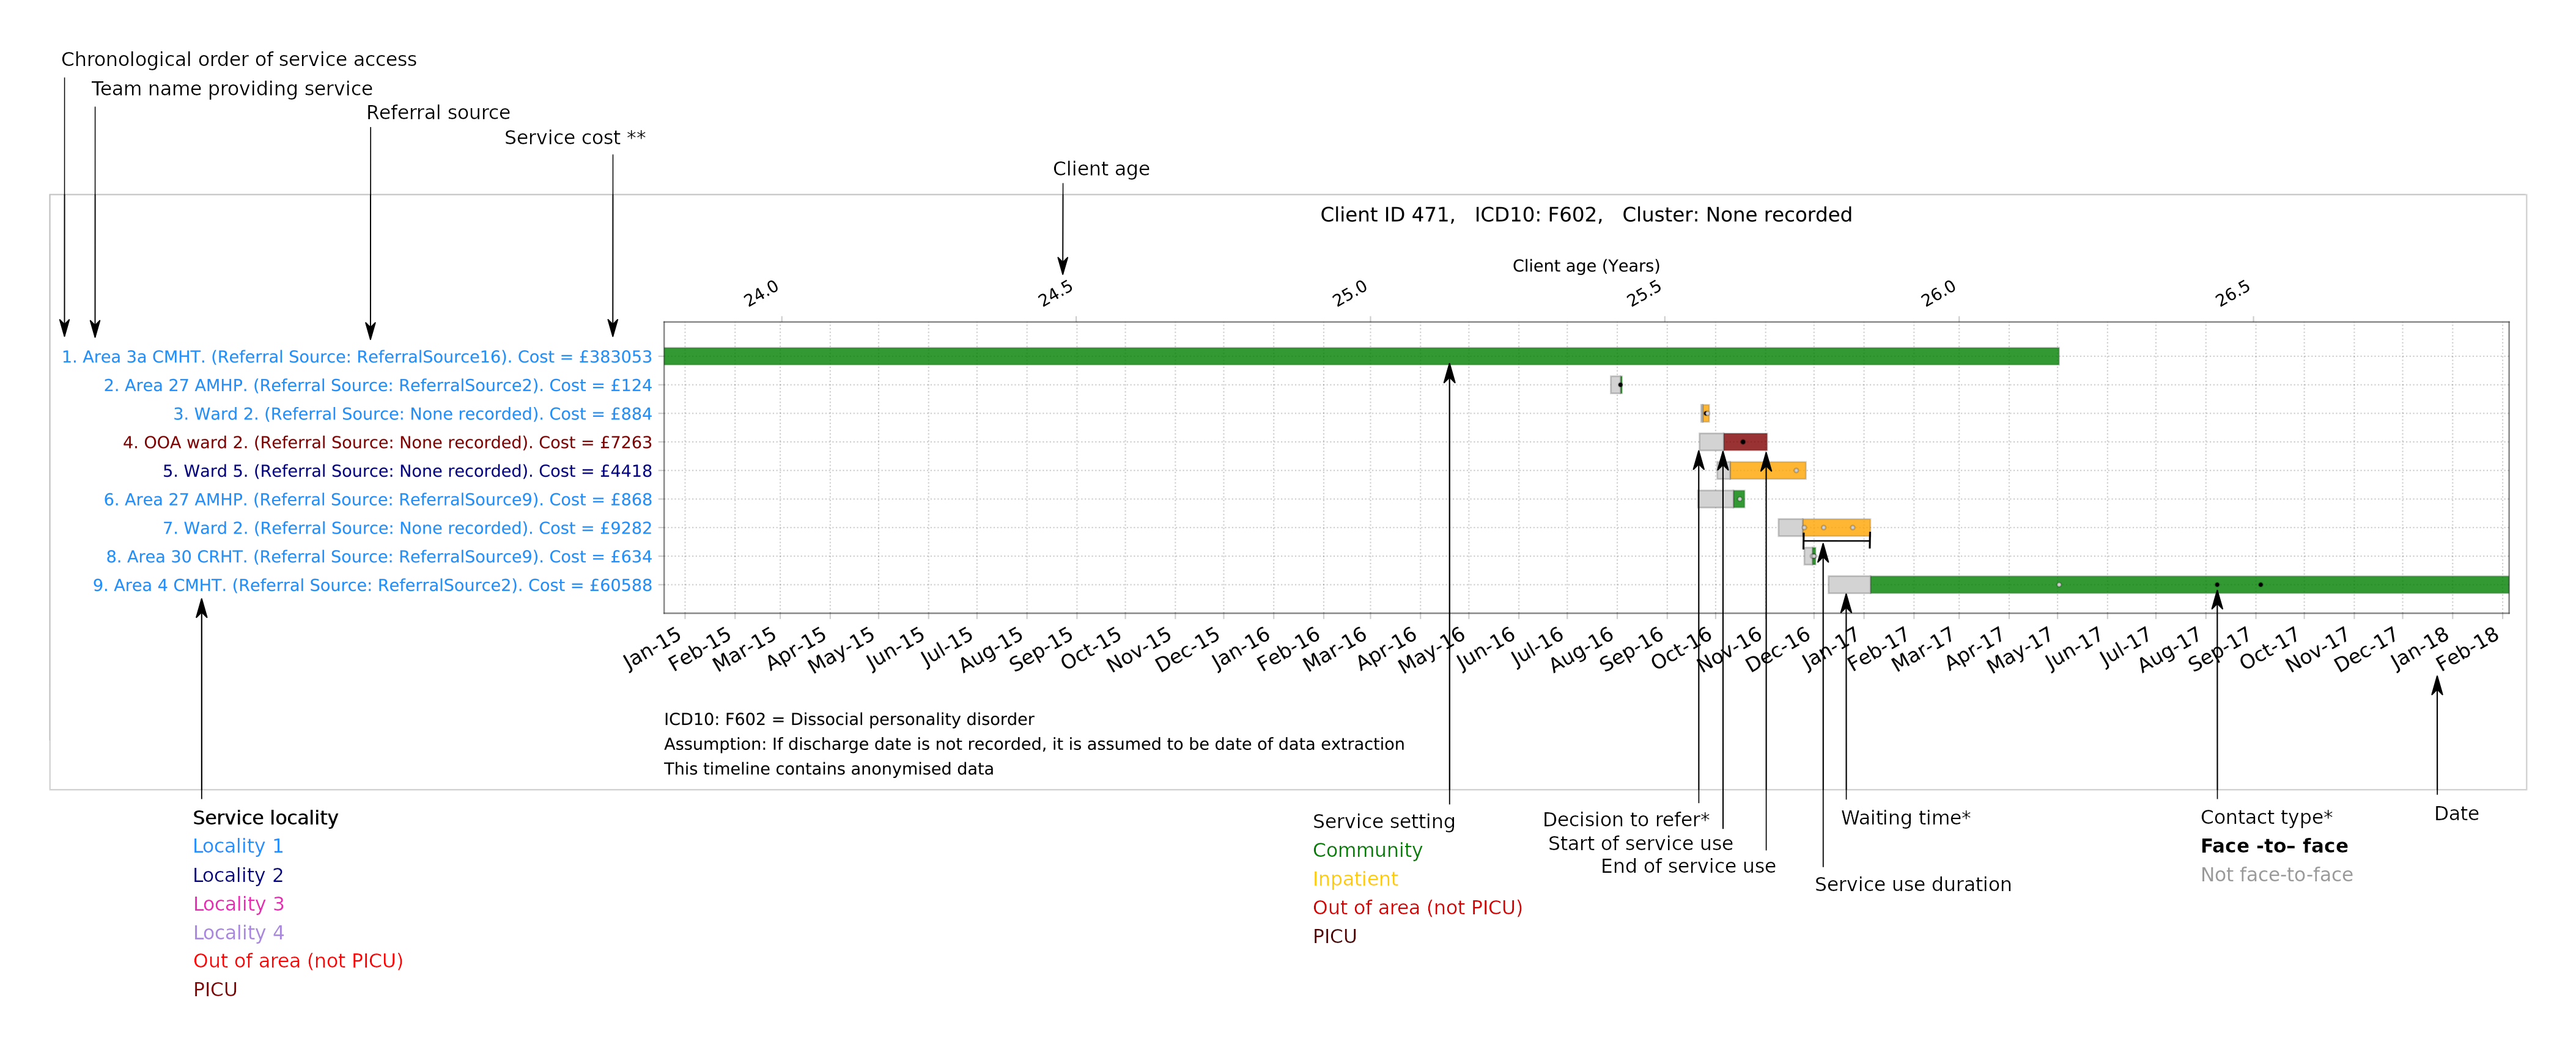
\includegraphics[width=0.9\textwidth]{images/200902_PD_service_use_timeline_471_figure.png}%200827_PD_service_use_timeline_figure_shutter.png}%SUT_for_paper.png}
	\caption{SUT for an individual PD client's service use, using data routinely recorded in Carenotes ( * \& ** indicate where surrogate data have been used to demonstrate proof of concept: * data recorded in Carenotes but were not included in the original data request; ** data not yet recorded in Carenotes).}
	\label{fig:sut}
\end{figure}


\section{Discussion}

Here we provide a link to Python code for visualisation of PD service use as SUT based on routinely collected service use data (Carenotes).

This study described the development of SUT, a visualisation tool, that at its core provides a clear and concise representation of the client’s mental health service use history as recorded in Carenotes. This tool aims to address some of the issues caused by the complexities and individual variation of treatment for clients diagnosed with a PD \cite{Bolton2014}. Particularly, we expect SUT may minimise instances of cyclical pathways, caused by referrals to services without a predefined treatment plan or clear understanding of client’s treatment history.
Compared to the traditional tabular format, the SUT displays the same information in a more readily accessible format, with the relative durations of each service used being clearly shown. Any overlaps of service use can easily be identified, as well as services that were used for a long period of time, or cyclical patterns of service use. The colour of the bars informs the clinician whether the client has been using mainly community services, or whether their care has been required to be escalated to an inpatient stay, or to a secure unit (PICU). Out of area services (depicted with a dark red bar) are easily identifiable, and the result of this stay on subsequent services used can be easily be seen – did the client require further inpatient services once they were returned to a service provided by the trust, or were they able to step down and use community services? 
In terms of treatment, having all of this information more readily available as a timeline can improve the clinicians understanding of the client’s clinical data, and help them to recognize complex patterns from the data, which will aid their ability to make clinical decisions \cite{Ledesma2019}. By making better referral choices for the client, this could reduce the number of services that the client will access, and for them to require fewer appointments, due to the client receiving the most appropriate care first. This would translate into  resource and financial savings for the services while improving patient care and experience.

While this tool was developed with particular focus on clients with a diagnosis of PD, the issues it address’s are common for other mental health conditions and potentially some chronic conditions, suggesting SUT could be extended to cover those services.

Some limitations of the SUT approach should be noted:
\begin{itemize}
	\item \emph{Data assumptions}: the graphic produced is only as good as the data. If any assumptions about the data are made, these need to be made visible to the user.
	\item \emph{Length of stay}: the length of stay is calculated from referral date to discharge date. This can be a long duration with minimal interaction between the client and the service. Anecdotally, clients are kept on the books for a particular service (usually a community service), if that service would like to ensure a future contact with the client. This highlights the lack of confidence some clinicians have in the current care pathway for a client with a PD diagnosis, as they are currently not confident the client will be referred back to the service if needed. Increased confidence in the system, could improve the accuracy with which length of stay is recorded. As demonstrated in this study, including contact instances as points within the service use bar can provide a more accurate indication of the intensity of interaction a client has with a service.
	\item \emph{Service use cost}: it was requested by DPT staff to include a service use cost for each service use episode. We attempted to calculate and include a value based on a service use cost per day, however at present, insufficient information is collected to calculate meaningful costs on which to base decisions. Utilising individual contact data rather than length of stay data would help to improve this calculation.
	\item \emph{Isolated view}: the medical and social care history of a client is more complicated than just their service use. People with a PD diagnosis will often be interacting with physical health services, social care and emergency services.  Including more data by creating linked datasets across different sectors  will enrich the knowledge that the clinician has about the client enabling a more informed decision.
	\item \emph{Overview}: the current visualisation is static, and as such can lose precise information (such as exact dates). Using some simple interaction techniques (such as tooltips) would help to overcome this.
	\item \emph{Computational time}: the current code calculates a data field that the plotting library (matplotlib) uses to define the location of that date on the graphic. This calculation is the most computationally expensive part of the code. For extensive use, and if time is a factor, an alternative method may be required.
\end{itemize}

Notwithstanding these limitations, the SUT are an improved method for visualising the data collected in Carenotes about the services a client has accessed. Using the SUT during consultations with clients can aid discussion, and help explore previous service use that did not have the desired outcome.

\section{Future work}

SUT has received a positive response from clinicians and plans are in place for DPT to electronically embed the SUT within their business intelligence tool – DUNDAS BMI. This is developed and maintained internally by DPT, and is linked to, and displays, up-to-date Carenotes data. As DPT internally manage DUNDAS BMI, this allows for the SUT to be updated as required to meet the needs of the clinicians (as they continue to be engaged in the process), alleviating barriers such as excessive cost \cite{Bidargaddi2018} and prohibitive licencing associated with third party software. 

The information displayed in SUT is only limited by the data recorded in Carenotes, the flexibility of the software and the developer’s availability. While this tool was developed with particular focus on clients with a diagnosis of PD, the issues it address’s are common for other mental health conditions (and potentially some chronic conditions), hence there are plans for SUT to be available for all mental health clients accessing DPT services.

The future design of the SUT should continue to be done in collaboration with the users (the clinicians and clients) to incorporate their preferences into the visualisation. When included in visualisation tool development, it was found that clinicians had clear preferences about the visualisation used, and appreciated the opportunity to be involved \cite{Gill2010}.

Future work is necessary to assess the impact of introducing these SUT to mental health service clinical decision making, and to understand if these translate into real world benefits for PD clients.

\section{Conclusions}

The code, and the SUT it creates, provides DPT clinicians with a useful tool to visualise their clients service use history (not restricted to just clients diagnosed with a PD).
If this method is adopted, and the same impact is achieved as other studies have reported, clinicians could benefit by spending less time understanding the data, and have a better recall of the information. This in turn can improve the decisions the clinicians make, putting clients on a more suitable care pathway for their needs, and improving the service’s ability to manage their resources as the clients are receiving more appropriate care.

\section*{Funding and acknowledgements}

This work was funded by Devon Partnership NHS Trust.

This study was supported by the National Institute for Health Research (NIHR) Applied Research Collaboration (ARC) South West Peninsula. The views and opinions expressed in this paper are those of the authors, and not necessarily those of the NHS, the NIHR, or the Department of Health and Social Care.

We thank Simon Wellesley-Miller and the DPT Informatics Team for the provision and knowledge of the Carenotes dataset.

\section{Conflict of interest statement}

Kerry Pearn declares no conflict of interest.\\
Dr Sean Manzi declares no conflict of interest.\\
Lindsay Winterton is an employee of Devon Partnership Trust who commissioned the research.

\section{References}

\bibliographystyle{ieeetr}
\bibliography{timelines_paper}
%\end{multicols}

\newpage
\section{Appendix}
The variables in the extracted Carenotes sample dataset

\begin{table}[h]
	\centering
	\caption{The variables in the extracted sample Carenotes dataset used to create the timelines}
	\begin{tabular}{
			p{\dimexpr.2\linewidth-2\tabcolsep-1.3333\arrayrulewidth}% column 1
			p{\dimexpr.6\linewidth-2\tabcolsep-1.3333\arrayrulewidth}% column 2
		}
		\toprule
		Variable name & Description
		\tabularnewline*
		\midrule
		ClientID & Unique code for each individual client \\
		Date\_of\_birth & Date of birth (format dd/mm/yyyy) \\
		ICD10 & ICD10 code \\
		Desc & ICD10 code description \\
		Cluster & Mental health care cluster number \\
		ReferralSource & Service that referred the client to this service use episode \\
		ReferralDate & Service use start date \\ 
		ReferralDischarge & Service use end date \\
		WardTeam & Name of team that provides the service \\
		Locality & Geographical locality of the service use \\
		GenSpecialty & General specialty of the service (for example: liaison psychiatry, psychotherapy, perinatal, eating disorder)\\
		Setting & Setting of the service use (community, inpatient, other local beds, out-of-area)\\
		OOABedType & The type of out of area service \\
		\bottomrule
		\label{tab:carenotes_variables}
	\end{tabular}
\end{table}

Additional variables added to the Carenotes sample dataset based on those requested by the stakeholders. These are mock variables created for the purposes of demonstration.

\begin{table}[h]
	\centering
	\caption{The requested variables created for the purposes of demonstration in the timelines}
	\begin{tabular}{
			p{\dimexpr.2\linewidth-2\tabcolsep-1.3333\arrayrulewidth}% column 1
			p{\dimexpr.6\linewidth-2\tabcolsep-1.3333\arrayrulewidth}% column 2
		}
		\toprule
		Variable name & Description
		\tabularnewline*
		\midrule
		RequestDate & Date this service was requested \\
		daily\_cost & Daily cost of the service use \\
		number\_contacts &  Number of individual contacts the client had with the service \\
		contact\_date\_1 & Date of first individual contact with service \\
		contact\_type\_1 &  Type of first individual contact with service (0 = face-to-face, 1 = not face-to-face) \\
		contact\_date\_2 &  Date of second individual contact with service \\
		contact\_type\_2 & Type of second individual contact with service (0 = face-to-face, 1 = not face-to-face) \\
		contact\_date\_3 & Date of third individual contact with service \\
		contact\_type\_3 & Type of third individual contact with service (0 = face-to-face, 1 = not face-to-face) \\
		contact\_date\_4 & Date of fourth individual contact with service \\
		contact\_type\_4 & Type of fourth individual contact with service (0 = face-to-face, 1 = not face-to-face) \\
		\bottomrule
		\label{tab:carenotes_variables}
	\end{tabular}
\end{table}

\newpage
The \textit{International Classification of Diseases (ICD-10) codes} are a global diagnostic tool.
Clients were included in the extracted Carenotes dataset if they had one of these twelve ICD-10 codes or a mental health care cluster 7 or 8.

\begin{table}[h]
	\centering
	\caption{ICD-10 code key}
	\begin{tabular}{
			p{\dimexpr.15\linewidth-2\tabcolsep-1.3333\arrayrulewidth}% column 1
			p{\dimexpr.45\linewidth-2\tabcolsep-1.3333\arrayrulewidth}% column 2
		}
		\toprule
		ICD-10 code & Description
		\tabularnewline*
		\midrule
		F60 & Specific personality disorders\\
		F60.0 & Paranoid personality disorder\\
		F60.1 & Schizoid personality disorder\\
		F60.2 & Dissocial personality disorder\\
		F60.3 & Emotionally unstable personality disorder\\
		F60.4 & Histrionic personality disorder\\
		F60.5 & Anankastic personality disorder\\
		F60.6 & Anxious [avoidant] personality disorder\\
		F60.7 & Dependent personality disorder\\
		F60.8 & Other specific personality disorders\\
		F60.9 & Personality disorder, unspecified\\
		F61 & Mixed and other personality disorders\\
		\bottomrule
		\label{tab:icd10}
	\end{tabular}
\end{table}

\textit{Mental health care clusters} provide a framework to plan and organise mental health care services for an individual. There are 21 mental health care clusters which broadly categorise clients into varying degrees of severity of: emotional difficulties; psychosis; memory difficulties \cite{NHSEnglandandNHSImprovement2019}. Clients were included in the extracted Carenotes dataset if they had a care cluster 7 or 8, or one of the ICD-10 codes listed above.  

\begin{table}[h]
	\centering
	\caption{Mental health care cluster key}
	\begin{tabular}{
			p{\dimexpr.15\linewidth-2\tabcolsep-1.3333\arrayrulewidth}% column 1
			p{\dimexpr.5\linewidth-2\tabcolsep-1.3333\arrayrulewidth}% column 2
		}
		\toprule
		Care cluster & Description
		\tabularnewline*
		\midrule
		7 & Enduring non-psychotic disorders (high disability)\\
		8 & Non-psychotic chaotic and challenging disorders\\
		\bottomrule
		\label{tab:icd10}
	\end{tabular}
\end{table}

\end{document}